%----------------------------------------------------------------------------------------
%							ustawienia dokumentu
%----------------------------------------------------------------------------------------

\documentclass[12pt, a4paper, oneside]{Thesis} % rozmiar czcionki,papieru, czy jednostronnie
\graphicspath{{./Pictures/}} % katalog z obrazkami

\usepackage[square, numbers, comma, sort&compress]{natbib} 
\hypersetup{urlcolor=blue, colorlinks=true} % kolory hiperlinków
\title{\ttitle} % Defines the thesis title - don't touch this

% włączenie polskich znaków
\usepackage[T1]{fontenc}
\usepackage[polish]{babel}
\usepackage[utf8]{inputenc}
\usepackage{lmodern}
\usepackage{graphicx}
\usepackage{wrapfig}

\selectlanguage{polish}


%==============================================================================================================
\begin{document}

\setstretch{1.5} % odstęp pionowy 

% Define the page headers using the FancyHdr package and set up for one-sided printing
\fancyhead{} % Clears all page headers and footers
\rhead{\thepage} % Sets the right side header to show the page number
\lhead{} % Clears the left side page header

\pagestyle{fancy} % Finally, use the "fancy" page style to implement the FancyHdr headers

\newcommand{\HRule}{\rule{\linewidth}{0.5mm}} % New command to make the lines in the title page

% PDF meta-data
\hypersetup{pdftitle=Kamil Lolo- praca inżynierska}
\hypersetup{pdfsubject=Praca inżynierska}
\hypersetup{pdfauthor=Kamil Lolo}
\hypersetup{pdfkeywords=Praca inżynierska}



%----------------------------------------------------------------------------------------
%								Strona tytułowa
%----------------------------------------------------------------------------------------

\begin{titlepage}
\begin{center}

%logo uniwersytetu
\begin{figure}
    \centering
    
\includegraphics[width=\linewidth]{./Pictures/logo.jpg}
\end{figure}

\textsc{\Large Inżynierska praca dyplomowa \newline }\\[0.5cm] 


{\huge \bfseries Platformowa gra zręcznościowa z wykorzystaniem biblioteki SDL }\\[0.4cm] % tytuł pracy

\addvspace{110pt}
 
\begin{minipage}{0.4\textwidth}
\begin{flushleft} \large
\emph{Autor:}\\
Kamil Lolo 
\end{flushleft}
\end{minipage}
\begin{minipage}{0.4\textwidth}
\begin{flushright} \large
\emph{Promotor:} \\
dr.Krzysztof Podlaski
\end{flushright}
\end{minipage}\\[3cm]


\vfill
\addvspace{20pt}
\begin{center}
Wydział Fizyki i informatyki stosowanej
\end{center}
{\large \today}\\[4cm] % Date


\end{center}
\end{titlepage}

%----------------------------------------------------------------------------------------
%								Spis treści
%----------------------------------------------------------------------------------------

% The page style headers have been "empty" all this time, now use the "fancy" headers as defined before to bring them back
\pagestyle{fancy}

% Set the left side page header to "Contents"

\lhead{\emph{Contents}} 

% Write out the Table of Contents
\tableofcontents 


%----------------------------------------------------------------------------------------
%									Rozdziały pracy
%----------------------------------------------------------------------------------------

% Rozpoczecie numerowania stron (1,2,3..)
\mainmatter 

% Return the page headers back to the "fancy" style
\pagestyle{fancy} 

% dołączanie poszczegolnych rozdzaiałów
% wstep
\setcounter{secnumdepth}{-1}
\renewcommand{\chaptername}{}
\lhead{\emph{Wstęp}}
\chapter{Wstęp} 
%----------------------------------------------------------------------------------------
Głównym celem tej pracy jest stworzenie gry która będzie działać w systemie Linuks, na który to obecnie jest nieporównywalnie mniej gier niż dla komercyjnego systemu Microsoft Windows. Linuks obecnie najczęściej znajduje zastosowanie jako oprogramowanie serwera, superkomputera. Rośnie jednak jego pozycja jako system dla komputerów biurkowych, chodź tutaj nadal uważany jest za system wyłącznie dla tzw. Geeków, czyli maniaków komputerowych z bardzo dużą wiedzą. Pogląd ten stopniowo zmieniany jest przez takie dystrubucje jak Ubuntu. Jest ona równie łatwy w użytkowaniu dla przeciętnego człowieka jak system Windows. Ciągle jednak Linuks nie cieszy się popularnością wśród graczy i twórców gier. Tendencja ta zaczęła się zmieniać w ciągu kilku ostatnich lat, czego dowodem może być wydanie na Linuksa przez firmę Valve Corporation systemu dystrybucji gier "Steam". Jest to niewątpliwie krok do przodu jeżeli chodzi o zmianę poglądu twórców gier że na Linuksa nie warto wydawać gier. Warto tutaj wspomnieć jeszcze o tym że Valve nie jest mało znaną firmą, bardzo wielu graczy kojarzy ją z grą Counter Strike, w którą przez kilka lat grały setki tysięcy ludzi na całym świecie.

Założenie że aplikacja ma działać natywnie w Linuskie. wykluczało użycie narzędzi nie kompatybilnych z tymże systemem, przykładem może być tutaj często wykorzystywany przy tworzeniu gier DirectX firmy Microsoft. Wybór padł natomiast na wieloplatformową bibliotekę Simple Direct Media Layer (w skrócie SDL) której lista docelowych platform jest bardzo długa.
Zaczynając od Linuksa, poprzez Windows, Mac OS aż do takich egzotycznych systemów jak Amiga OS. Dodatkową zaletą biblioteki SDL jest fakt że stanowi ona wolne oprogramowanie open source na licencji „zlib”. SDL posiada także kilka dodatkowych bibliotek stanowiących rozszerzenie jej możliwości. W aplikacji zostaną wykorzystane dodatkowe moduły rozszerzające API SDL-a o obsługę
dźwięku oraz czcionek. Nie są to jednak wszystkie dostępne wtyczki do SDL-a, warto wspomnieć też o bibliotece SDL\_Net dzięki której możliwe jest stworzenie gry sieciowej. Najważniejszymi możliwościami jakimi dysponuje SDL jest utworzenie kontekstu graficznego i obsługa zdarzeń, biblioteka pozwala również za pomocą zestawu funkcji renderować obraz. Rysowanie za pomocą SDL-a często okazuje się jednak zbyt wolne, twórcy biblioteki pozwolili obejść ten problem poprzez wykorzystanie do renderowania 
niskopoziomowej biblioteki OpenGL, która również jest kompatybilna z Linuksem.

Następnym założonym celem aplikacji było wykorzystywanie zewnętrznych skryptów (tzw. skryptowanie) które dawałyby możliwość manipulowania pewnymi danymi aplikacji bez potrzeby jej re-kompilacji. Skrypty te będą napisane w języku Lua, który został zaimplementowany w ANSI C, dzięki czemu zapewnia wysoką wydajność i przenośność na wiele platform. Ogromnym plusem połączenia programu napisanego w C++ oraz Lua jest to że z poziomu aplikacji C++ można wywoływać funkcje zadeklarowane w skrypcie, a mogą one być zmieniane bez potrzeby rekompilacji aplikacji. Funkcje umieszczone w skrypcie są uruchamianie podczas działania aplikacji przez maszynę wirtualną Lua. Cały ten mechanizm działa również w drugą stronę z poziomu skryptu Lua można wywołać funkcję C++, co też zostanie wykorzystane w aplikacji.

Stworzona na potrzeby pracy gra będzie posiadać grafikę 2D, a dedykowanym systemem operacyjnym będzie linuks, chodź dzięki zastosowaniu wieloplatformowych narzędzi pozostaje możliwość uruchomienia jej w innych systemach np. Microsoft Windows, bądź też Mac OS. Warto tutaj wspomnieć także o mobilnym systemie Blackberry  który to wspiera wszystkie technologie które będą użyte w pracy. Daje to możliwość umieszczenia gry w Black Berry App Word – markecie z aplikacjami na urządzenia mobilne z tymże systemem. Co wiąże się z możliwością zarobienia pieniędzy na tej grze. Reasumując. W pracy zostanie przedstawiona aplikacja pokazująca możliwości SDL-a jako biblioteki do tworzenia gier. Przedstawiona zostanie również możliwość wykorzystania skryptów w języku Lua jako narzędzia pozwalającego przenieść część logiki aplikacji poza skompilowany
program.
%----------------------------------------------------------------------------------------


\setcounter{secnumdepth}{1}
\renewcommand{\chaptername}{Rozdział}
%============================================================================================================================
%							 						Fabuła
%============================================================================================================================
\chapter{Wprowadzenie} 

\section{Fabuła}
\lhead{Rozdział 1. \emph{Fabuła}}

Celem gracza będzie przebiec jak największy dystans. Będzie to bieg astronauty przez obcą planetę na której musi zbierać bańki z tlenem oraz omijać przeszkody żeby nie zginąć. Przeszkodami takimi będą meteoryty zmniejszające poziom życia. Astronauta podczas gry będzie cały czas biec do przodu,zwalniając jedynie w przypadku niskiego poziomu życia.

\begin{wrapfigure}{left}{0.5\textwidth}
\begin{center}

\includegraphics[width=120px]{./Pictures/astro.jpg}
\end{center}
\caption{Postać astronauty }
\label{Etykieta}
\end{wrapfigure}

Poziom życia będzie ciągle spadał, i bańki z tlenem będą go zwiększać. 
Gracz będzie miał możliwość podskakiwania astronautą oraz wznoszenia się nim do góry Sporadycznie na mapie będą się pokazywać bonusy który astronauta będzie mógł zebrać (maksymalnie 3 naraz) i wykorzystać później do uzupełnienia ilości życia. Taki bonus będzie dawał także nieśmiertelność przez kilka sekund, wtedy to na brzegach ekranu pojawi się charakterystyczna obwódka. Kiedy gracz zakończy grę, wtedy jego wynik, czyli ilość przebytych metrów zapisywany będzie na liście 10 najlepszych wyników. Wyniki te będą zapisywane w osobnym pliku na dysku, tak żeby dane nie zostały stracone po wyłączeniu aplikacji. Listę najlepszych wyników będzie można obejrzeć wybierając z głównego menu pozycje „highscore”. Ze względu na fabułę z biegnącym
astronautą, oraz osadzenie zdarzeń na obcej planecie, gra została nazwa „Astro Rush”.


%============================================================================================================================
%							 						 Grafika
%============================================================================================================================
\section{Grafika}
\lhead{Rozdział 1. \emph{Grafika}}

Grafika w grze będzie się opierać o tzw. sprite. Technika ta polega na tworzeniu animacji, bądź też rysowania dużych obrazów z serii małych obrazków
które zazwyczaj są fragmentami jednej grafiki. Poszczególne klatki animacji biegu astronauty przedstawia na rysunek 2.

\begin{figure}[h]
    \centering
    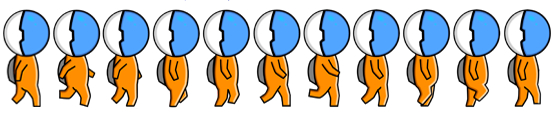
\includegraphics[width=0.8\textwidth,natwidth=410,natheight=142]{./Pictures/astroRun.jpg}
    \caption{Animacja biegu astronauty}
\end{figure}

Wszystkie animacje w grze są przechowywane w jednym głównym pliku „atlas.png”. Skąd wyświetlany jest tylko fragment odpowiadający danemu sprite-owi.
Po upływie określonego czasu następuje przejście do następnej klatki animacji, czyli zazwyczaj przesuniecie współrzędnej X o szerokość obrazka. W tym
algorytmie współrzędna Y nie zmienia się. Cały algorytm wyświetlania animacji opartej przestawia schemat 1.
Warto tutaj wspomnieć o układzie współrzędnych jaki jest używany w bibliotece SDL. Otóż punkt początkowy (0,0) znajduje się w lewym górnym
rogu, prawy górny wierzchołek to ( szerokośćokna, 0 ), natomiast lewy dolny to : (0, wysokość okna ). Grafika na potrzeby gry została częściowo
stworzona w edytorze grafiki wektorowej Inkscape, który oparty jest na licencji GPL i działa pod takimi systemami operacyjnymi jak np. Windows, Linux.
Narysowanie części obrazków jako grafiki wektorowej pozwoliło zachować pełną skalowalność w dalszym procesie tworzenia grafiki. Utworzone grafiki
wektorowe były składane i poprawiane w Adobe Photoshop – bardzo rozbudowanej aplikacji do obróbki grafiki rastrowej. Photoshop jest aplikacją płatną,
jednak istnieje możliwość użycia 30 dniowej wersji Trial, co też zostało zrobione podczas tworzenia gry. W atlasie grafiki znalazły się także ikony z
kolekcji „Hand drawn icon set” które autor opublikował w internecie  na darmowej licencji.

\begin{figure}[h]
    \centering
    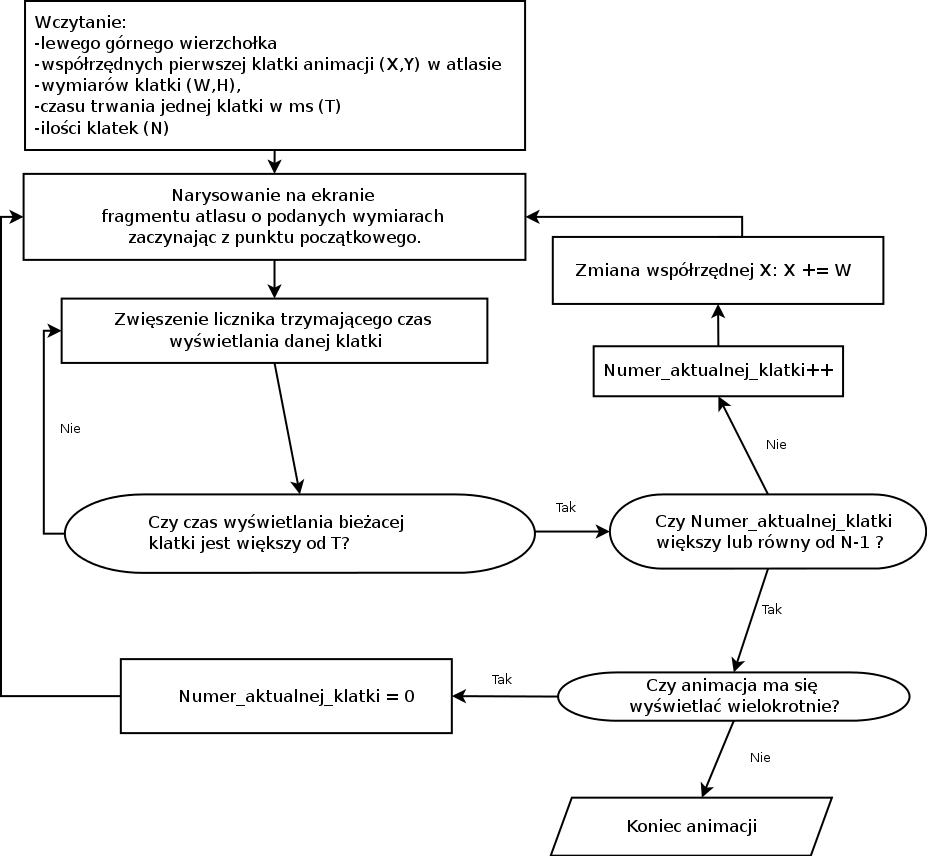
\includegraphics[width=0.8\textwidth,natwidth=410,natheight=142]{./Pictures/sprite_algorytm.png}
    \caption{Schemat wyświetlania animacji opartej o sprite}
\end{figure}


%============================================================================================================================
%							 						Eclipse
%============================================================================================================================
\section{Użyte narzędzia}

\lhead{Rozdział 1. \emph{Użyte narzędzia}}
\subsection{Eclipse}
Środowiskiem w którym będzie powstawać aplikacja będzie Eclipse IDE. Znane jest ono przede wszystkim jako bardzo dobre narzędzie do pisania aplikacji
w Javie, ale dzięki doinstalowaniu wtyczki CDT (C/C++ Development tooling) można w nim rozwijać projekt w języku C++. Eclipse posiada integracje z
wieloma przydatnymi narzędziami, które czasami bardzo upraszczają życie programiście. Przy tworzeniu Astro Rush były wykorzystane:
-Integracja Eclipse z debuggerem. W tym przypadku znany konsolowy gdb.
Najbardziej przydatna okazała się tutaj możliwość zatrzymania programu na breakpoincie oraz sprawdzenie stosu wywołań.
-Integracja z make, co zostanie omówione w kolejnym podrozdziale
-Możliwość doinstalowania kolejnych wtyczek. Przy tworzeniu przydatna
okazała się wtyczka aplikacji Valgrind jako narzędzie do wykrywania wycieków pamięci, oraz integracja z aplikacją Perf. Jest to profiler który
pokazuje statystyki odnośnie tego które wywołania metod trwają najdłużej. Profilowanie okazało się pomocne podczas refactoringu w ramach którego
została przeprowadzona optymalizacja wydajności.


%============================================================================================================================
%							 							Make
%============================================================================================================================
\subsection{Make}
Eclipse jako platforma programistyczna dedykowany jest językowi Java, a kolejne wtyczki pozwalające pisać w innych językach to tylko rozszerzenie tego
środowiska Javy. Eclipse z wtyczką do języka C++ może używać programu Make, który automatyzuje budowanie projektu składającego się z wielu plików.  
Zostało to wykorzystane w projekcie. Ogromnym plusem takiego rozwiązania jest to żeby zbudować aplikacje nie potrzeba ściągać Eclipse-a, ale wystarczy
make, który zajmuje niewiele miejsca na dysku i jest wieloplatformowy. Dodatkowo bardzo łatwo się go instaluje w większości dystrybucji Linuksa. Make
korzysta z pliku reguł domyślnie o nazwie „makefile”. Taki plik dla omawianej gry wygląda następująco:

\begingroup
\fontsize{10pt}{12pt}\selectfont
\begin{verbatim}  
CXX = g++
CFLAGS = -Wall -ansi -pedantic -g -std=c++0x -Wall -I ./include -O0 -c

# flagi linkera
LIBS = -lGL -lGLU -lSDL -lSDL_mixer -lSDL_ttf -lSDL_image -lluabind -llua5.1

# lista plikow źródłowych do kompilacji
SOURCES = src/main.cpp src/App.cpp src/Property.cpp src/Resource.cpp 

# jak maja się nazywać skompilowanie pliki cpp
OBJECTS=$(SOURCES:.cpp=.o)

# nazwa pliku wynikowego
EXECUTABLE = AstroRush.bin

# domyslny cel dla wywolania make bez argumentu, czyli zbudowanie projektu
all: $(SOURCES) $(EXECUTABLE)

# linkowanie aplikacji
$(EXECUTABLE): $(OBJECTS)
	 @echo "\n ---- Linkowanie ---- "
	$(CC) $(OBJECTS) -o $(EXECUTABLE) $(LIBS)

#kompilowanie plikow cpp
.cpp.o:
	 @$(CXX) $(CFLAGS) $< -o $@

# czyszczenie aplikacji przed zbudowaniem  
clean:
	rm -rf ./src/*.o
	rm ./AstroRush.bin 
    \end{verbatim}  
\endgroup

Domyślne wywołanie make bez żadnych parametrów spowoduje zawsze uruchomienie domyślnego celu budowania: all. Możliwe jest definiowania dowolnej ilości
celów budowania w jednym makefile-u. W grze został dodany również cel do czyszczenia gry z wszystkich skompilowanych źródeł oraz zlinkowanej
aplikacji, co okazuje się przydatne kiedy występuje potrzeba przebudowania projektu, bowiem make sprawdza czasy ostatniej modyfikacji  plików tzw.
timestampy i kompiluje tylko te źródła które uległy zmianie od ostatniej kompilacji.
	W napisanym na potrzeby gry pliku „makefile” widać że w plikach makefile można definiować swoje własne zmienne, tutaj na przykład zmienną są
flagi linkera, kompilatora, oraz lista plików źródłowych z katalogu src. Tak napisany makefile jest bardzo uniwersalny i kolejne nowe pliki wymagają
jedynie dopisania ich na listę źródeł. Ewentualnie podczas kompilacji w systemie w którym w zmiennej środowiskowej nie ma kompilatora g++ można tutaj
podać ścieżkę gdzie ten kompilator się znajduje.
	Budowanie aplikacji poprzez make bądź też podobne narzędzie o nazwie cmake jest wyjątkowo popularne w systemie Linuks i projektach napisanych
w języku C/C++. Make jest nawet wykorzystywany do budowania jądra Linuksa, które składa się z milionów linii kodu ( wersja 3.2 to w przybliżeniu 15
mln ) oraz setek plików, gdzie nie wszystkie muszą być skompilowane, a przy rekompilacji kompilowane są tylko te które uległy zmianie, dzięki czemu
oszczędność czasu przy kompilacji jest znacząca.


%============================================================================================================================
%														Git
%============================================================================================================================
\subsection{Git}
Projekt Astro Rush nie wydaje się zbyt duży biorąc pod uwagę fakt że nie przekroczył 10 tysięcy linii kodu. Jednak zawsze warto mieć jakąś kopie na
repozytorium oraz ewentualnie możliwość poprzez historie  zmian przywrócenie jakiś fragmentów kodu. Narzędziem które okazało się tutaj pomocne jest
rozproszony system kontroli wersji – git. Darmowe oprogramowanie stworzone przez Linusa Torvaldsa do zarządzania kodem jądra Linuksa. Git jest również
narzędziem wieloplatformowym, chodź pod systemem Windows jest on wolniejszy niż na Linuksie. Przy tworzeniu aplikacji został wykorzystany serwis
hostujący gita: https://github.com/. Hosting dla aplikacji open source jest darmowy, jednak w takim przypadku repozytorium z kodem jest publiczne.
Warto wspomnieć o tym że serwis github mimo tego że powstał dość nie dawno bo w 2008, ma już 2 miliony repozytoriów.
	Podczas tworzenia aplikacji została wykorzystana wtyczka do eclipse która pozwala w łatwy sposób synchronizować projekt który znajduje się na
dysku lokalnie z tym co jest na repozytorium, oraz wysyłanie zmian na serwer.


\section{OpenGL jako silnik grafiki}
\lhead{Rozdział 1. \emph{OpenGL jako silnik grafiki}}

%============================================================================================================================
%											 Czym jest OpenGL
%============================================================================================================================
\subsection{Czym jest OpenGL}
Open Graphics Library (w skrócie OpenGL) jest niskopoziomową biblioteką  graficzną 3D. Kompatybilny jest on z większością liczących się systemów
operacyjnych, został on także zaimplemtowany na urządzeniach mobilnych, przykładem może być tutaj JOGL, czyli Java-owa wersja OpenGL-a której można
używać na urządzeniach z systemem Android. OpenGL jest często wykorzystywany jako podstawowe API przy tworzeniu silników do gier 3D przykładem może
być tutaj choćby nawet silnik ID tech znany min. z serii gier Quake . Mimo że OpenGL jest przystosowany do pracy z grafiką trójwymiarową to doskonale
można go wykorzystać do grafiki 2D, tak jak to miało miejsce w grze Astro Rush. OpenGL posłużył do wyświetlania tekstur na ekranie, co odbywało się
zdecydowanie szybciej niż poprzez funkcje do rysowania z biblioteki SDL.  Różnica w szybkości renderowania wynosiła około 20 fps-ów na sekundę na
laptopie hp550 z procesorem dual core 1.4 ghz. OpenGL dostarcza także takich zaawansowanych elementów jak obsługa cieni oraz oświetlenia, jednak z
racji wykorzystania grafiki 2D nie znalazło to zastosowania w projekcie.
	W bardzo łatwy sposób można połączyć SDL-a i OpenGL-a.
W SDL podstawowym elementem graficznym na którym odbywa się rysowanie jest powierzchnia (ang. surface). Podczas inicjowania biblioteki SDL tworzona
jest główna powierzchnia na której następnie będzie się odbywać rysowanie ( często też nazywane w grafice 2D „blitowaniem” ). Podczas inicjowania
głównej powierzchni ekranu żeby używać do renderowania OpenGL-a wystarczy poprzez funkcje SDL\_SetVideoMode podać flagę SDL\_OPENGL. Trzeba jeszcze
pamiętać żeby po każdym rysowaniu wywołać funkcję: SDL\_GL\_SwapBuffers() która wysyła bufor ramki do rysowania na ekranie.


%============================================================================================================================
%							 Wykorzystanie OpenGL do renderowania grafiki w grze
%============================================================================================================================
\subsection{Wykorzystanie OpenGL do renderowania grafiki w grze}
SDL posiada rozszerzenie SDL\_image które umożliwia obsługę różnych formatów grafiki (w grze zostały wykorzystane pliki graficzne o rozszerzeniach png oraz jpeg). Pozwala one w łatwy sposób wczytać plik z dysku poprzez funkcje SDL\_Surface *IMG\_Load(const char *file) , która zwraca surface z
wczytanym obrazkiem. SDL\_Surface jest strukturą w której znajduje się wskaźnik do pamięci gdzie znajduje się wczytana z dysku grafika. Ten adres (
„void* pixels” ) należy przekazać jedynie do OpenGL-a podczas tworzenia tekstury.
Można w ten sposób rysować nie tylko pliki graficzne wczytane z dysku ale również obiekty graficzne utworzone w aplikacji. Taka sytuacja ma miejsce w
przypadku renderowania napisów, gdzie jest tworzony surface z napisem, i następnie rysowany za pomocą OpenGL-a. W aplikacji proste prymitywy graficzne
jak prostokąty wypełnione kolorem są rysowane również za pomocą API OpenGL-a.


%============================================================================================================================
%											Skrypty w języku Lua
%============================================================================================================================
\section{Skrypty w języku Lua}
\lhead{Rozdział 1. \emph{Skrypty w języku Lua}}
Lua jest lekkim językiem skryptowym zaprojektowanym do rozszerzania możliwości innych aplikacji. Został on zaimplementowany w języku C zgodnie ze standardem ANSI, zapewnia mu to przenośność na wiele platform. Najważniejszym cechami tego języka jest to że jest dynamicznie typowany, oraz obiektowy. Jest on wykorzystywany zarówno do tworzenia rozszerzeń do różnych aplikacji, co często nazywane jest skryptowaniem (ang.scripting) oraz jako samodzielny język, w którym skrypty będą wykonywane poprzez maszynę wirtualną Lua. Samo skryptowanie wiąże się z ideą programowania sterowanego danymi (ang. data driven development).
Podejście te zakłada że wszelkie stałe kontrolujące zachowanie programu oraz wybrane elementy logiki powinny być zdefiniowane poza program. W aplikacji skrypty Lua są wykorzystywane do przechowywanie wszystkich ustawień, oraz obliczania pewnych wartości 
już w czasie działania aplikacji.Przykładowo rozmiar gracza jest obliczany na poziomie skryptu przy wykorzystaniu ustawionych podczas działania gry zmiennych z rozmiarami ekranu. 

\begin{figure}[h]
    \centering
    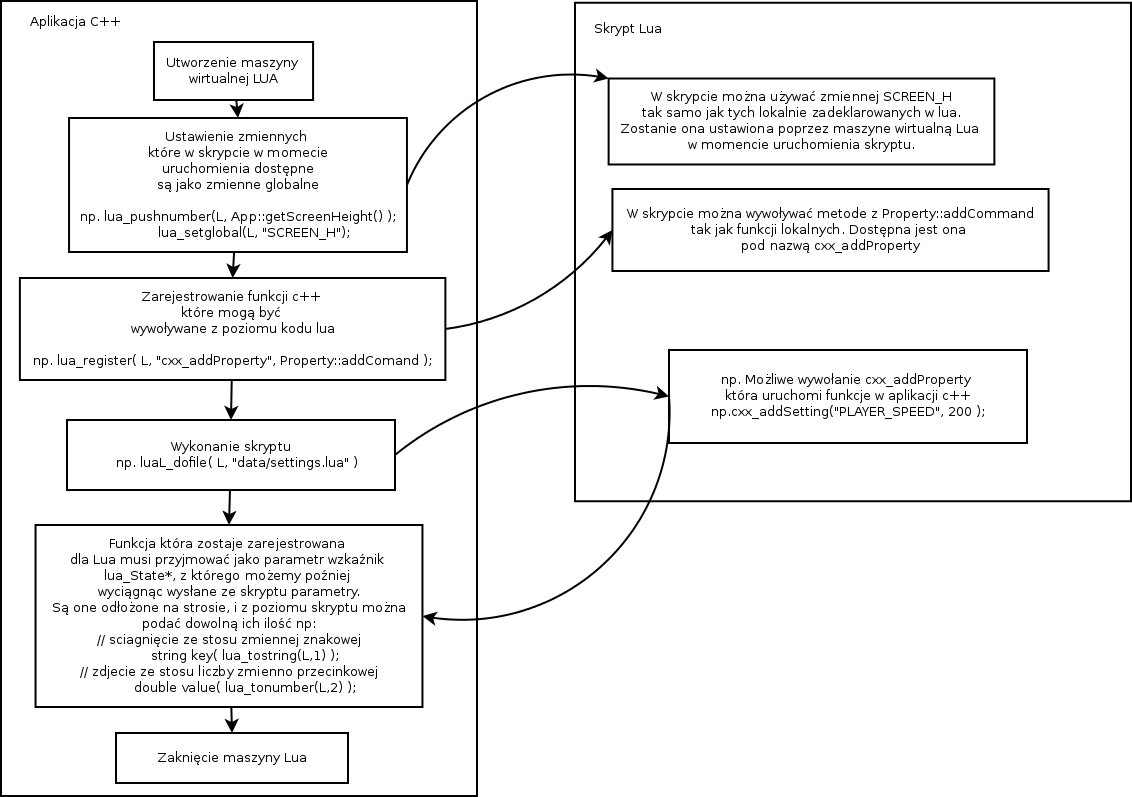
\includegraphics[width=0.8\textwidth,natwidth=410,natheight=142]{./Pictures/lua_skrypty.png}
    \caption{Przepływ danych między aplikacją C++ a skryptem Lua}
\end{figure}

Powyższy rysunek pokazuje przykładowy przepływ danych między aplikacją C++ a skryptem Lua. Wykorzystane tu zostało wywołanie funkcji C++ z poziomu skryptu, aczkolwiek w drugą stronę ten mechanizm również działa. To znaczy z poziomu C++ można wykonać funkcje Lua. Lua została wykorzystana do internacjonalizacji aplikacji. Podobnie jak to jest wykorzystywane w aplikacjach webowych w języku Java, gdzie wszystkie komunikaty są przechowywane w plikach properties. Podczas uruchamiania aplikacji zostaje odczytany odpowiedni plik dla danego języka. Cały proces ilustruje rysunek 5. W rezultacie takiej budowy aplikacja może działać z dowolnym językiem. Podczas tworzenia zostały napisane komunikaty zarówno polskie jak i angielskie.


%============================================================================================================================
%											Obsługa czcionek
%============================================================================================================================
\section{Obsługa czcionek w SDL}
\lhead{Rozdział 1. \emph{Obsługa czcionek w SDL}}
W projekcie została wykorzystana biblioteka SDL\_ttf pozwalająca używać w aplikacji czcionek w formacie True Type. Format ten stworzony przez firmę Apple przechowuje kształty poszczególnych liter jako krzywe Beziera, i jest on obsługiwany przez większość platform. Na Linuksie jest on bardzo powszechnym formatem do obsługi czcionek, dodatkowym plusem jest ogromna ilość czcionek na darmowych licencjach. W grze została wykorzystana czcionka "Ubuntu" udostępniona za darmo, i będąca domyślną czcionką w dystrybucji Linuksa o tej samem nazwie. Plik z taką czcionką (standardowo o rozszerzeniu *.ttf) jest wczytywany podczas uruchamiania aplikacji, następnie poprzez wywołania funkcji z biblioteki SDL\_ttf np. TTF\_RenderUTF\_Blended zostaje utworzona powierzchnia na której narysowany jest napis o podanej treści, kolorze oraz rozmiarze. 

Niestety powierzchnia taka jest zwracana jako wskaźnik na strukturę SDL\_Surface, przez co konieczna jest konwersja na format obsługiwany przez OpenGL-a. Niedogodność taka nie występowałaby gdyby do renderowania było wykorzystywane API biblioteki SDL. Identyczny problem występuje również przy renderowaniu innych elementów graficznych które są ładowane z dysku i zwracane jako SDL\_Surface* (Wczytywanie takie realizowane jest poprzez kolejną bibliotekę będącą uzupełnieniem SDL-a: SDL\_image. Służy ona do wczytywania plików graficznych w takich formatach jak np. JPEG, PNG, TIFF. W aplikacji wykorzystana jest tylko jedna funkcja 
z tej biblioteki stąd też nie będzie ona szerzej omawiana).

Sama konwersja SDL\_Surface* na GLuint to wygenerowanie tekstury w standardowy dla OpenGL-a sposób, wykorzystując przy tym pole pixels ze struktury SDL\_Surface, które jest adresem pod którym przechowywane są poszczególne piksele obrazka. W uproszczeniu funkcja realizująca taką konwersje w grze wygląda następująco:

\begingroup
\fontsize{10pt}{12pt}\selectfont
\begin{verbatim}  
void RendererGL::create_gl(SDL_Surface * surf, GLuint * tex )
{
 
   /** ...tutaj określenie ilości kolorów i formatu */
  
    glGenTextures( 1, tex );
    glBindTexture( GL_TEXTURE_2D, *tex );

    /** ...tutaj ustawienia parametrów tekstury */

    glTexImage2D( GL_TEXTURE_2D, 0, colors_amount,
    			  	surf->w, surf->h, 0, format, 
    			 	 GL_UNSIGNED_BYTE, surf->pixels );
}
\end{verbatim}
\endgroup

Warto wspomnieć że biblioteka SDL\_ttf pozwala renderować napisy z polskimi znakami, o ile takie występują w wczytanej czcionce. Ponadto SDL\_ttf dostępny jest podobnie jak SDL na darmowej licencji zlib, i jest wieloplatformowy jak wszystkie wtyczki do SDL-a. W niektórych dystrybucjach zainstalowanie tej biblioteki, oraz innych wspomnianych bibliotek rozszerzających SDL-a sprowadza się do wykonania jednego polecenia- zainstalowania pakietu z repozytorium. Dla dystrybucji Debian oraz jego pochodnych będzie to polecenie:
\begin{verbatim}
apt-get install libsdl-ttf2.0-dev 
\end{verbatim}

\chapter{Budowa aplikacji} 
%============================================================================================================================
%							 						Glowna petla
%============================================================================================================================

\section{Główna pętla}
\lhead{Rozdział 2. \emph{Główna pętla}}

W grach komputerowych często wykorzystywane jest tzw. programowanie sterowane zdarzeniami. Polega ono na umieszczeniu w aplikacji głównej pętli, w której to cyklicznie będzie się odbywać obsługa zdarzeń (np. naciśniecie klawisza ), aktualizacja gry oraz rysowanie. Sama kolejność tych elementów nie odgrywa większej roli, warto natomiast zwrócić uwagę na to że po zatrzymaniu pętli następuje przygotowanie aplikacji do wyłączenia. W przypadku Atsro Rush po wyjściu z głównej pętli zatrzymywany jest kontekst graficzny SDL-a, zwalniane są wszystkie zajęte zasoby, i następuje wyłączenie gry. Pętla taka najczęściej implementowana jest jak while, którego zakończeniem steruje flaga wyjścia. Przy każdym obiegu pętli wartość tej flagi wyciągana jest z klasy Game, która to decyduje kiedy należy zakończyć działanie aplikacji. 

\begin{figure}[h]
    \centering
    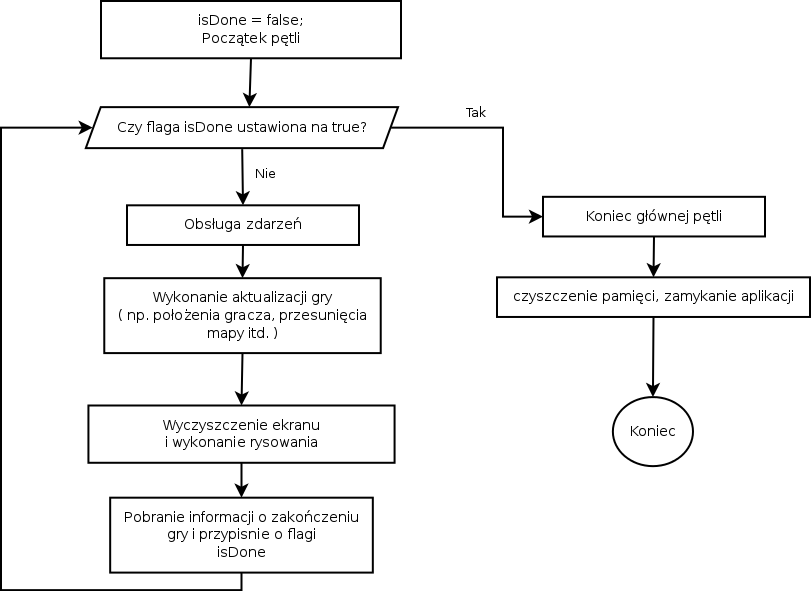
\includegraphics[width=0.8\textwidth,natwidth=410,natheight=142]{./Pictures/main_loop.png}
    \caption{Schemat działania głównej pętli}
\end{figure}

Pętla stanowi najważniejszy element większości gier, to od niej zależy czy gra będzie działać tak samo na urządzeniach różniących się wydajnością. W projekcie pętla jest dość prosta i oprócz typowych elementów typu aktualizacja, rysowanie, obsługa zdarzeń, uwzględnia jedynie sytuacje w której całość obliczeń i rysowań odbywa się zbyt szybko i należy wykonać opóźnienie. Taki problem może się pojawić na szybszych urządzeniach na których gra działała by zbyt szybko. W przypadku bardziej złożonej aplikacji można także uwzględnić sytuacje odwrotną, kiedy to ostatnia aktualizacja stanu gry odbywała się zbyt wolno i w następnym obiegu pętli należy wykonać aktualizacje kilkukrotnie żeby zapobiec braku płynności w renderowanym obrazie. Taka sytuacja jednak w grze Astro Rush nie powinna mieć miejsca z racji tego iż jest jest to gra z grafiką dwuwymiarowa i występują w niej proste obliczenia matematyczne.


%============================================================================================================================
%							 						Mapa kafelkowa
%============================================================================================================================
\section{Mapa w grze}

\lhead{Rozdział 2. \emph{Mapa kafelkowa}}
\subsection{Mapa kafelkowa}
Mapa kafelkowa (ang. tiled map) jest jedną z podstawowych technik przy tworzeniu gier z grafiką dwuwymiarową. Technika ta polega na podziale świata dostępnego w grze na fragmenty (tzw. kafelki ) o tych samych rozmiarach. Najczęściej są to kwadraty, którym przypisujemy odpowiednie identyfikatory grafik. Tak utworzona mapa przechowywana jest w postaci dwuwymiarowej macierzy w osobnym pliku na dysku, i jest wczytywana podczas startu aplikacji w osobnym wątku. Macierz składająca się wyłącznie z cyfr (typu short żeby dodatkowo oszczędzić pamięć) zajmuje o wiele mniej pamięci w przeciwieństwie do rozwiązania w którym  z dysku wczytywana jest cała mapa w postaci jednej grafiki. Na podstawie tej macierzy rysowana jest mapa widoczna na ekranie. 

Z racji tego że gracz ciągle wędruje prze mapę, ta cały czas jest przesuwana, a dokładniej  to inkrementowany jest indeks kolumny w macierzy kafelków od której zaczynamy rysowanie. Kolumna o takim indeksie rysowana jest na ekranie jako pierwsza z lewej strony, następnie rysowane są obok (po prawej stronie) kolejne kolumny aż do momentu w którym mapa pokrywa cały ekran.
Kolumna od której zaczyna się rysować od lewego brzegu ekranu przesunięta jest w lewo o pewien offset, który zwiększnay jest podczas biegu gracza do przodu. Offset ten sprawia że współrzędna na osi X skrajnej kolumny zostaje przesunięta w lewo po za ekran, tak że widoczny jest tylko fragment kolumny na ekranie. Przejście do następnej kolumny następuje w momencie kiedy skrajna kolumna znajduje się całkiem po za ekranem. Dzięki zastosowaniu takiego algorytmu nastepuje płynne przesuwanie mapy, bez widocznych przeskoków pomiędzy kolejnymi kolumnami.
 

%============================================================================================================================
%							 						Edytor leveli
%============================================================================================================================
\subsection{Edytor mapy}
\lhead{Rozdział 2. \emph{Edytor mapy}}
Opisana w poprzednim podrozdziale macierz kafelków w grze Astro Rush ma wymiary: 30000 x 15. Stąd też pojawił się problem edycji tak dużej ilości danych. Zmiana poszczególnych wpisów ręcznie nie wchodziła w grę, dlatego też powstała dodatkowa aplikacja do edycji mapy. W wizualny sposób, z wykorzystaniem jedynie myszy można w niej stworzyć w kilkanaście minut całą mapę, rozmieszczając na niej dostępne rodzaje kafelków. Edytor umożliwia także wczytanie stworzonej wcześniej mapy i jej edycje. Aplikacja została napisana z wykorzystaniem biblioteki Qt udostępnionej na licencji LGPL. Biblioteka ta jest zestawem przenośnych narzędzi do tworzenia między innymi interfejsu użytkownika, obsługi sieci, grafiki trójwymiarowej (OpenGL), plików i wielu innych. 


\begin{figure}[h]
    \centering
    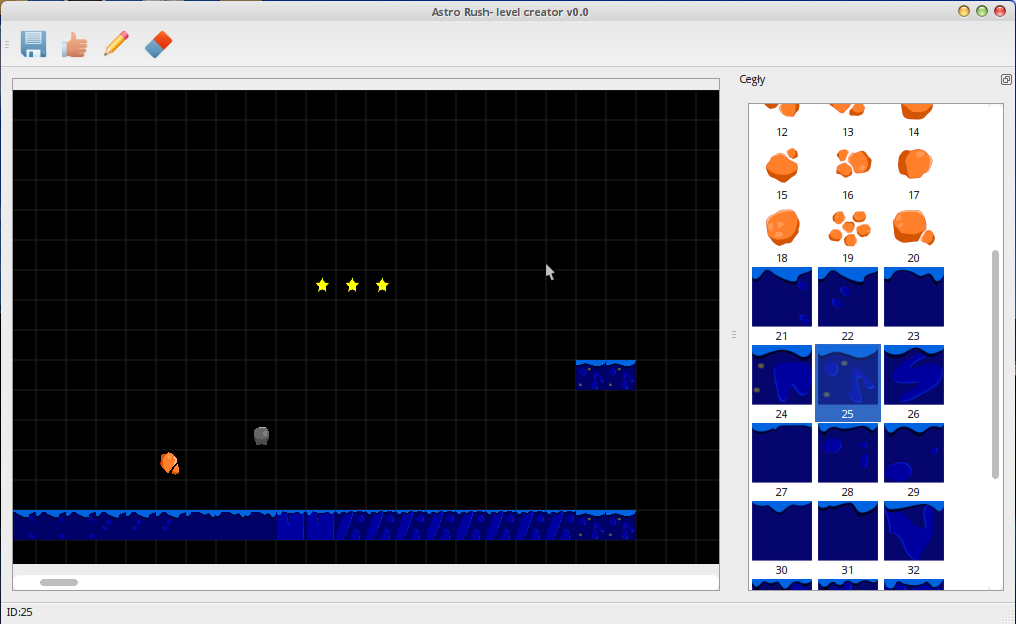
\includegraphics[width=0.8\textwidth,natwidth=800,natheight=142]{./Pictures/designer.png}
    \caption{Edytor mapy podczas pracy}
\end{figure}

Edytor mapy wyświetla całą planszę w postaci siatki na której naniesione są kafelki. Poprzez kliknięci w daną komórkę możemy zmienić rodzaj kafelka który w danym miejscu ma się wyświetlić, bądź też wyczyścić daną komórkę. Do pliku zapisywane są tylko numery odpowiadającym poszczególnym kafelkom, na bazie których gra rozpoznaje jaką grafikę w danym miejscu wstawić. Numeracja kafelków rozpoczyna się od 0, natomiast wartość -1 oznacza że w danym miejscu nie ma kafelka i taki fragment nie jest rysowany.

%============================================================================================================================
%							 						Uruchamianie aplikacji
%============================================================================================================================
\section{Uruchamianie aplikacji}
\lhead{Rozdział 2. \emph{Uruchamianie aplikacji}}
sdfd



%============================================================================================================================
%							 						Warstwy aplikacji
%============================================================================================================================
\section{Warstwy aplikacji}
\lhead{Rozdział 2. \emph{Warstwy aplikacji}}

Lorem ipsum dolor sit amet, consectetur adipiscing elit. Duis eu massa ante. Maecenas pretium metus a libero commodo convallis. Mauris a dignissim lacus. Cum sociis natoque penatibus et magnis dis parturient montes, nascetur ridiculus mus. Duis eleifend magna ut magna commodo dapibus. In adipiscing enim eget sapien elementum et adipiscing ligula sagittis. Curabitur ullamcorper cursus vulputate. Donec dignissim, tortor eget adipiscing rhoncus, risus mauris varius nisi, ac vehicula elit orci sit amet nunc. Fusce massa nisi, imperdiet vitae volutpat non, euismod ullamcorper lectus. Mauris iaculis sagittis tortor, quis convallis elit luctus eu. Sed sodales viverra velit, quis porttitor ipsum vulputate nec.









\chapter{Dokumentacja użytkownika} 
%============================================================================================================================
%							 	Sterowanie w grze
%============================================================================================================================
\section{Sterowanie w grze}
\lhead{Rozdział 1. \emph{Fabuła}}
Astronauta w grze biegnie ciągle do przodu, a osoba sterująca nim ma możliwość wykonania skoku poprzez naciśniecie klawisza spacja. W przypadku kiedy gracz chce wykonać krótki skok, tzn. nie może poczekać aż bohater przestanie się wznosić wtedy z pomocą przychodzi klawisz Ctr którym zatrzymujemy ruch pionowy kosmonauty. Zatrzymanie następuje na ułamek sekundy, jednak naciskając bardzo szybko ten klawisz można sprawić, że bohater leci prawie poziomo. Może się to okazać pomocne przy przelatywaniu przez jakieś tunele na mapie. 


\begin{wrapfigure}{left}{0.5\textwidth}
\begin{center}

\includegraphics[width=170px]{./Pictures/ilosczycia.png}
\end{center}
\caption{Licznik bonusów}
\label{Etykieta}
\end{wrapfigure}

Podczas biegu na mapie można zebrać bonusy które przywracając pełna ilość życia i sprawiają, że życie te nie opada przez kilka sekund. Po znalezieniu takie bonusu w lewym górnym rogu pojawia się informacja o tym. Maksymalnie można mieć 3 niewykorzystane bonusy, i podczas działania jednego nie da się uruchomić kolejnego, co zapobiega zbyt szybkiemu wytraceniu wszystkich znalezionych dodatków. Znaleziony bonus można aktywować poprzez wciśniecie lewego klawisza shift. Po aktywowaniu bonusu dokoła ekranu pojawia się niebieska otoczka oznaczająca nieśmiertelność. 


%============================================================================================================================
%Menu
%============================================================================================================================
\section{Menu}
\lhead{Rozdział 1. \emph{Fabuła}}
Główne menu zostało zaprojektowane w programie do tworzenia grafiki rastrowej Adobe Photoshop. Z jego poziomu można rozpocząć nową grę, kontynuować bieżącą, obejrzeć klawiszologie, oraz listę najlepszych wyników w formie tabelki. Możliwość konstytuowania bieżącej gry staje się aktywna w momencie kiedy gracz podczas gry nacisnął klawisz escape co za skutkowało wyjściem do głównego menu, oraz zamrożeniem bieżącej rozgrywki. Nawigacja w menu odbywa się wyłącznie za pomocą klawiatury. Klawisz strzałka w górę przechodzi do następnej pozycji powyżej, strzałka w dół działa natomiast odwrotnie. Aktualnie wybrany element menu podświetlany jest za pomocą koloru pomarańczowego, nie aktywny kolorem szarym, a domyślny białym. Zatwierdzenie wybranej opcji następuje poprzez wciśniecie klawisza enter, co stanowi standardową nawigacje w większości menu do gier. Naciśnięcie klawisza w głównym menu spowoduje zamknięcie aplikacji. 

\begin{figure}[h]
    \centering
    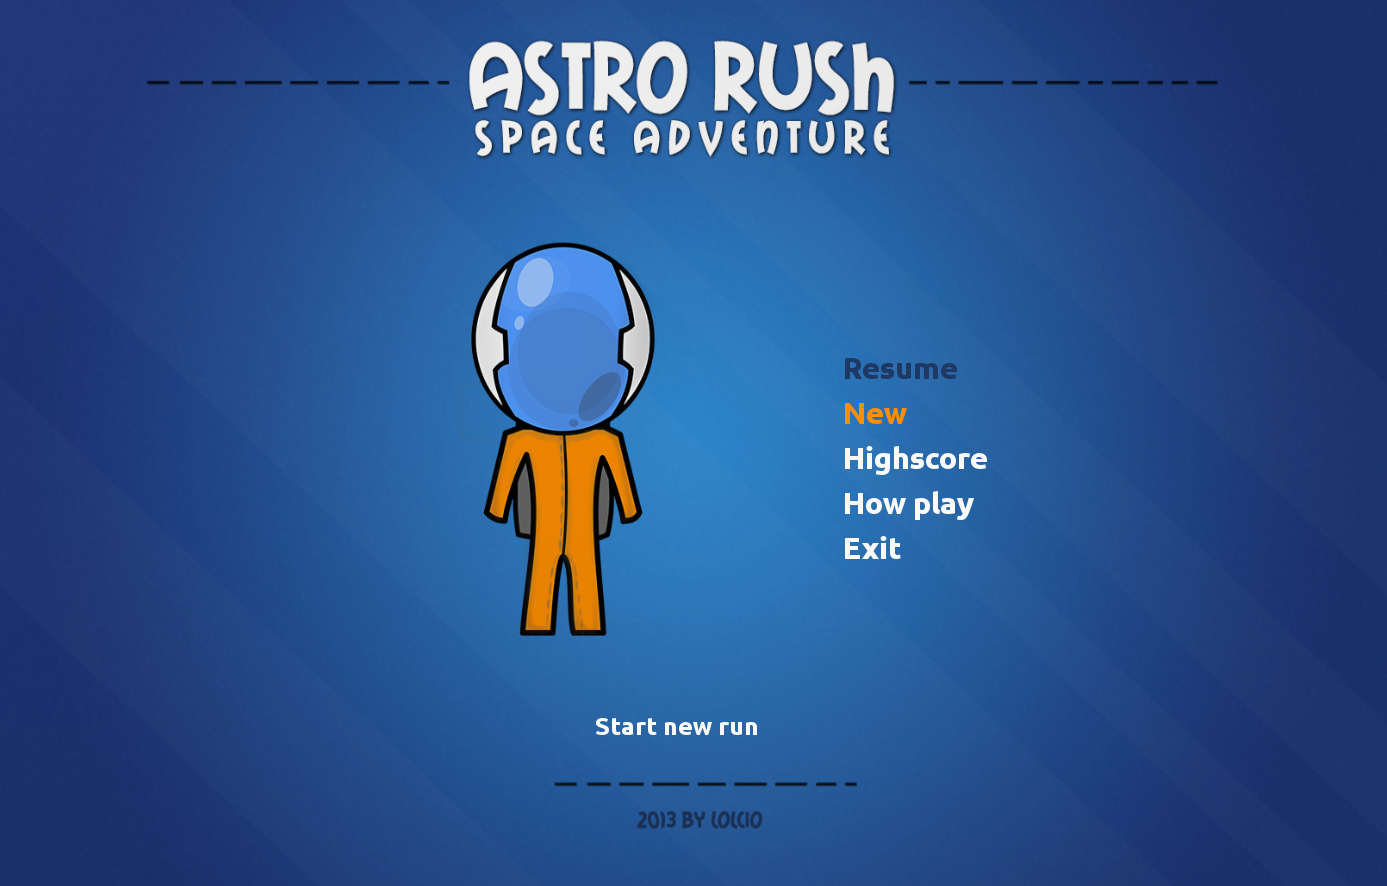
\includegraphics[width=429px]{./Pictures/menu1.png}
    \caption{Menu główne gry}
\end{figure}

\newpage 

\begin{figure}[h]
    \centering
    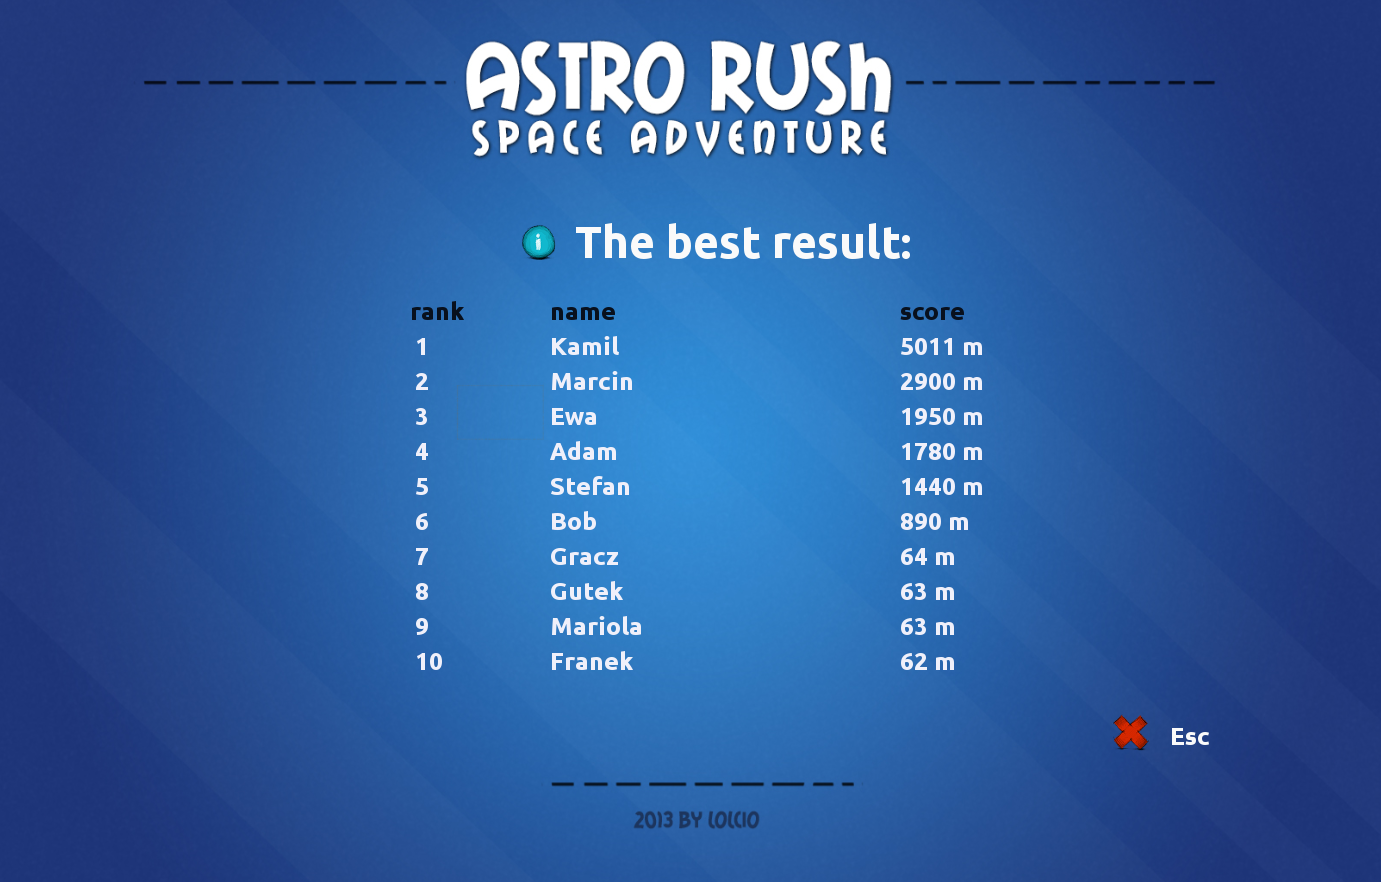
\includegraphics[width=429px]{./Pictures/menu2.png}
    \caption{Highscore w grze}
\end{figure}


\begin{figure}[h]
    \centering
    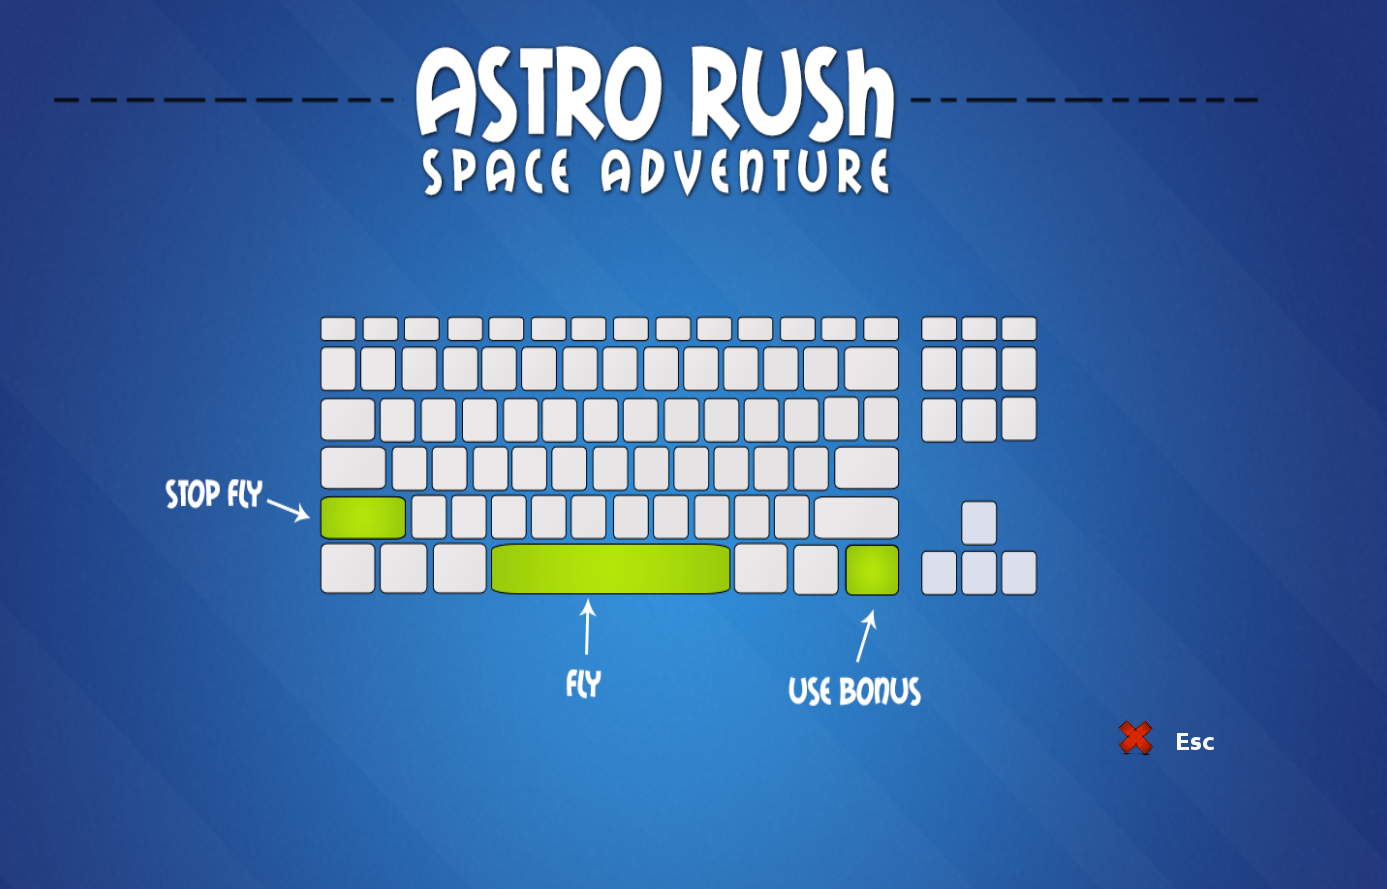
\includegraphics[width=429px]{./Pictures/menu3.png}
    \caption{Klawiszologia dostępna poprzez menu główne w grze}
\end{figure}


%============================================================================================================================
%							 		Instalacja
%============================================================================================================================
\section{Instalacja}
\lhead{Rozdział 1. \emph{Fabuła}}
W tym rozdziale zostanie przedstawiona instalacja potrzebnych bibliotek oraz kompilacja aplikacji na przykładzie systemu Debian. W przypadku innych wersji systemu Linuks nie bazujących na Debianie instalacja ta może wyglądać inaczej np. w systemie Fedora gdzie nazwy pakietów są inne, oraz ścieżka do biblioteki SDL jest inna. Dla Fedory kompilacja aplikacji wymaga zmian ścieżek do bibliotek w pliku Headers.hpp. Dlatego też w przypadku wersji aplikacji która miała by być dostarczona szerszemu gronu odbiorców konieczne jest przygotowanie rozwiązania unifikującego proces kompilacji pod różnymi dystrybucjami Linuksa. Innym rozwiązanie może przygotowanie prekompilowanych pakietów dla najpopularniejszych platform np. deb i rpm. Dodatkowym problemem może okazać się brak niektórych pakietów w repozytorium i konieczność ręcznego ich ściągania, jednak taka sytuacja nie powinna mieć miejsca z racji tego, że wykorzystane biblioteki są popularne wśród twórców gier dla Linuksa. 

W systemie Debian żeby zainstalować wymagane pakiety należy najpierw odświeżyć listę pakietów poleceniem: 

\begin{verbatim}
	aptitude update
\end{verbatim}

W przypadku braku aplikacji aptitude można użyć analogicznie apt-get. Następnym krokiem jest zainstalowanie wymaganych bibliotek w wersji developerskiej w przypadku samodzielnej kompilacji:
\begin{verbatim}
	aptitude install libsdl-1.2-dev lisdl-ttf2.0-dev libsdl-sound1.2-dev 
					 libsdl-mixer1.2-dev libsdl-image1.2-dev libluabind-dev 
					 liblua5.1-0-dev
\end{verbatim}

Jeżeli instalacja przebiegła bez problemów to wtedy można przystąpić do kompilowania gry.
W katalogu z rozpakowanym kodem należy wykonać polecenie make i poczekać aż pojawi się informacja o udanym zbudowaniu programu. W przypadku komputerów z wielordzeniowym procesorem można zoptymalizować proces budowania podając parametr -j<tutaj\_liczb\_rdzeni>.

W przypadku kiedy budowanie się nie powiedzie i pojawią się błędy, należy doinstalować brakujące biblioteki bądź też zmienić ścieżki do bibliotek. Ewentualnie oczyszczenie projektu z już skompilowanych plików można wykonać za pomocą polecenia "make clean". 

Po zakończeniu budowania zostanie utworzony plik AstroRush.bin (nazwa ta jest zdefiniowana w pliku makefile). Należy nadać mu prawo wykonywania:
\begin{verbatim}
chmod +x ./AstroRush.bin
\end{verbatim}

A następnie można uruchomić aplikacje. W przypadku Linuksa należy pamiętać żeby program był uruchamiany na partycji zamontowanej z prawem do wykonywania aplikacji. Często domyślnie urządzenia przenośne nie mają ustawionego takiego prawa. 
% wstep
\setcounter{secnumdepth}{-1}
\renewcommand{\chaptername}{}
\lhead{\emph{Zakończenie}}
\chapter{Zakończenie} 
%============================================================================================================================
%Zakończenie
%============================================================================================================================
\hspace{1cm} W pracy została przedstawiona budowa platformowej gry zręcznościowej mogącej pracować w systemie Linuks, gdzie brakuje gier oraz w najpopularniejszym obecnie systemie dla komputerów osobistych- Windows. 
Gra została stworzona w oparciu o własny silnik, pokazujący możliwości biblioteki SDL. Zaczynając od możliwości stworzenia i zarządzania oknem, poprzez integracje z OpenGL aż do obsługi dźwięku oraz czcionek. Omówiona biblioteka nie ustępuje możliwością bibliotece DirectX, której ogromnym ograniczeniem jest brak wsparcia dla systemu Linuks. Ponadto aplikacja pokazuje przykładowa budowę gry w której do renderowania grafiki wykorzystuje się sprite-y oraz mape kafelkową. Techniki te są jednymi z najbardziej podstawowych zagadnien w grach opartych o grafike dwuwymiarową.

W pracy został poruszony temat rozszerzenia możliwości programu w oparciu o tzw. skryptowanie. Zaprezentowane skrypty w języku Lua stanowią obecnie wtyczki rozszerzające funkcjonalonść nie tylko w grach, lecz wszędzie tam gdzie przeniesienie pewnych informacji poza skompilowany program pozwala oszczędzić czas potrzebny na jego napisanie.  

Stworzona aplikacja nie musi być tylko programem napisanym do pracy dyplomowej, może zostać ona upowszechniona jako projekt Open Source. Nie wykluczone jest, że wtedy będzie dalej rozwijana przez osoby chętne do wolontariatu. Udostępnienie kodu jako darmowego pozwala również na stworzenie pakietu prekompilowanego dla systemu Debian ( Plik z rozszerzeniem deb) i zgłoszenie go do repozytorium dystrybucji Debian, bądź Ubuntu. 

Inną możliwością co do przyszłością programu jest sprzedawanie gry jako tzw. Indie Game czyli gry niezależnej, stworzonej bez wsparcia finansowego przez jedną bądź kilka osób. Taką aplikacje można sprzedawać w formie elektronicznej za niewielkie pieniądze. Aplikacja może zostać uruchomiona na tablecie z systemem BlackBerry i umieszczona w markecie z aplikacjami dla tego systemu. Mowa jest tutaj szczególnie o tabletach ponieważ aplikacja podlega ograniczeniom odnośnie rozdzielczości ekranu na którym może zostać uruchomiona, co zostało opisane bardziej szczegółowo w pracy.  

Efektem ubocznym stworzenia gry Astro Rush było stworzenie silnika gry 2D. Silnik ten dzięki zastosowaniu zewnętrznych skryptów podatny jest na modyfikacje i zmianę. Prosta budowa pozwala na stworzenie na bazie bieżącej aplikacji kolejnej gry. Użycie biblioteki OpenGL do renderowania grafiki daje możliwość stworzenia dużo bardziej zaawansowanej grafiki, wykorzystującej cieniowanie i oświetlenie. 




\lhead{\emph{Spis ilustracji}} % Set the left side page header to "List of Figures"
\listoffigures % Write out the List of Figures

\addtocontents{toc}{\vspace{2em}} % Add a gap in the Contents, for aesthetics
\backmatter

%----------------------------------------------------------------------------------------
%									Bibliografia
%----------------------------------------------------------------------------------------
\begin{thebibliography}{1}

\bibitem{sop}Janusz Ganczarski. 
\emph{OpenGL w praktyce}. Wydawnictwo BTC, 2008.

\bibitem{sop}Stephan Pazera. 
\emph{Focus o SDL}. Wydawnictwo ???

\end{thebibliography}
\end{document}


\end{document}  
